% !TeX root = ./11-handout.tex

%\item<2-> % reveals second and keeps on page in subsequent frames
%\begin{itemize}[<2->] %does for a whole list of items

%could do reductio proofs! 
%changes to notion of rigor in mathematics; e.g. bolzano moving away from physical intuition , motion, passage of time. 



\setcounter{section}{10} 

\section{Certainly, Probably, Possibly? Unlikely!}
%\subsection*{test}

\begin{frame}
%\large

\scriptsize{\tableofcontents}

\end{frame}

%\iffalse %start of day one stuff 


\begin{frame}
\frametitle{Liable to forget:}
%\large

\begin{itemize}[<+->]

\item No more PSets ever! 
\item[] (for this class; bammmmm domain restriction!)

\item Good luck with finals and projects!!!! 

%\item no office hours this week

\item Evals are still live! 

%\item[] -- Upload screenshots of BOTH completion pages to earn: % the following:

\item[] -- 1 freebie recitation absence (so $\sim$a gradepoint)

\item[] -- 0.75 points back to Lecture Attendance total

\item Mega thanks to all of you who have completed them!!!! 
%\item[] -- (so if you attempt 15pts worth of a question on PSet 9 or 10, you'd get full points)


\end{itemize}
\end{frame}

\begin{frame}
  \frametitle{Happy Birthday to our boy Russell on Thursday!}

  \begin{columns}
    \begin{column}{.5\textwidth}
      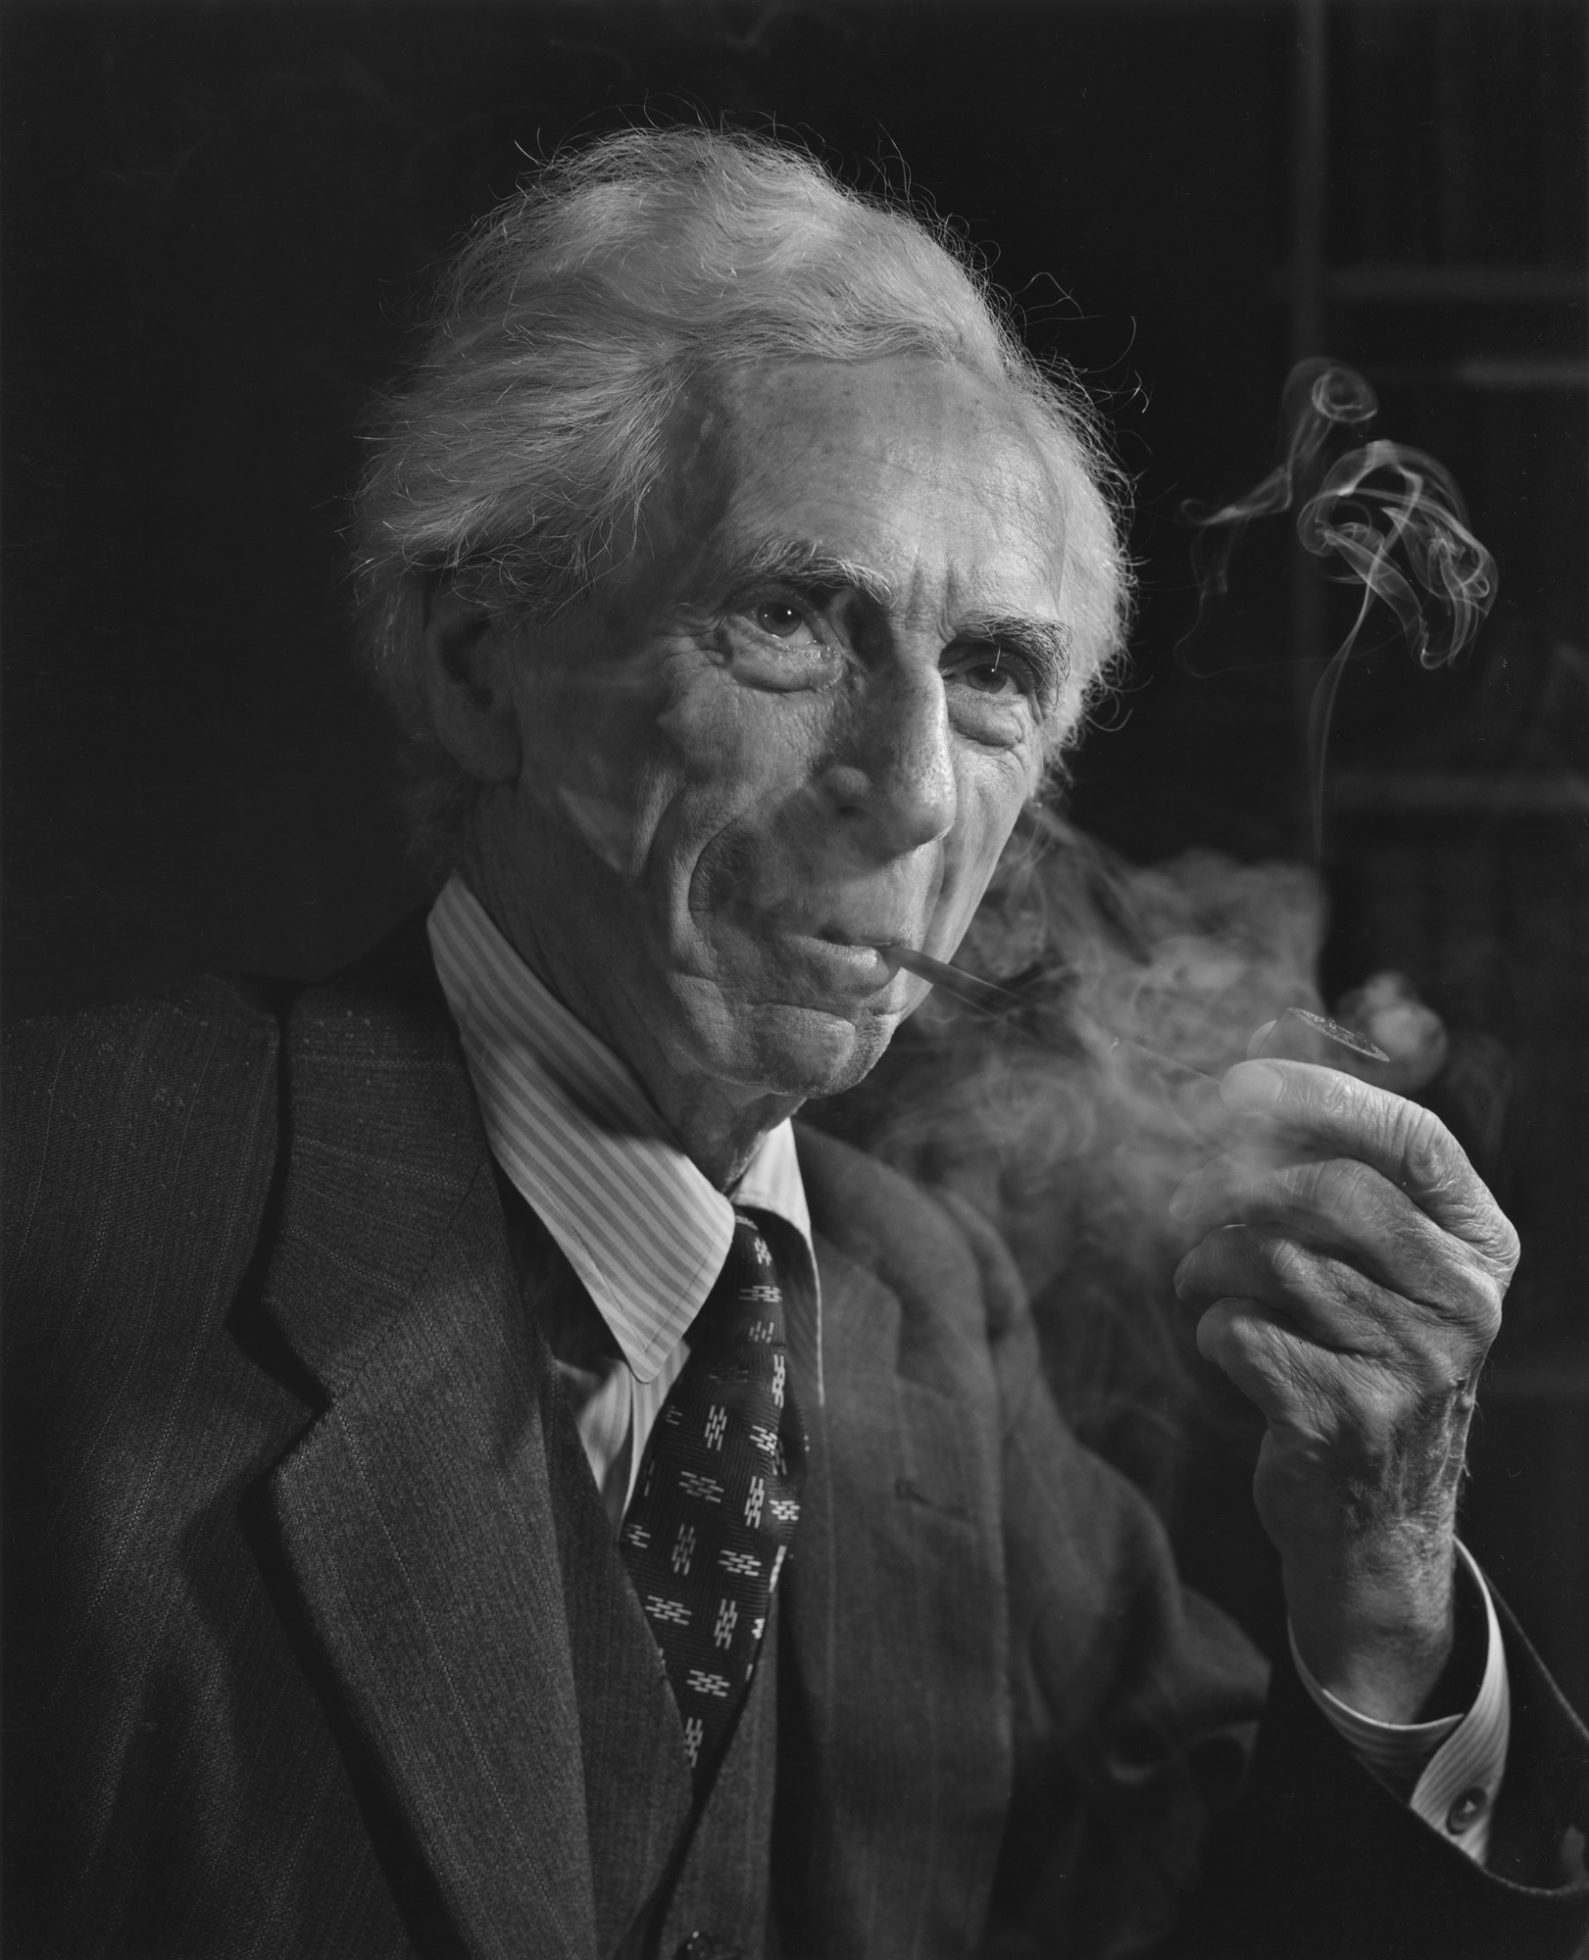
\includegraphics[height=.8\textheight]{../assets/russell_pipe}
    \end{column}
    \begin{column}{.6\textwidth}
      \begin{itemize}[<+->]
        \item Bertrand Russell \\ (a.k.a. 3rd Earl Russell) \\ (May 18th, 1872--1970)
       % \item Giant of 20th century philosophy!
\item A founder of analytic philosophy!

\item qua logician, attempted with Whitehead to reduce math to logic 

\item Also a pacifist and political activist 

\item Teacher of Wittgenstein
      \end{itemize}
    \end{column}
  \end{columns}
\end{frame}

\begin{frame}
  \frametitle{Happy Birthday to Wang on Saturday!}

  \begin{columns}
    \begin{column}{.5\textwidth}
      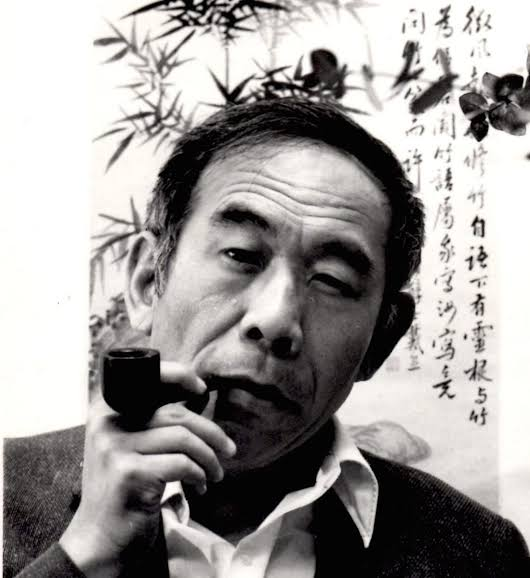
\includegraphics[height=.8\textheight]{../assets/wang}
    \end{column}
    \begin{column}{.6\textwidth}
      \begin{itemize}[<+->]
        \item Hao Wang \\ (May 20th, 1921--1995)
       % \item Giant of 20th century philosophy!
\item Logician and philosopher 

\item 1959: early work in automated theorem proving

%fun tidbit in relation to russell above haha: ``In 1959, Wang wrote on an IBM 704 computer a program that in only 9 minutes mechanically proved several hundred mathematical logic theorems in Whitehead and Russell's Principia Mathematica.''

\item Key commentator on G\"odel \\ (and Wittgenstein)

\item Inventor of Wang tile

%from wiki: 11the domino problem asks whether there is an effective procedure that correctly settles the problem for all given domino sets,'' i.e. whether we can effectively determine whether any given dominoe set (i.e. set of Wang tiles) will tile the plane with a period pattern.
% Wang's student Berger ``proved that no algorithm for the problem can exist, by showing how to translate any Turing machine into a set of Wang tiles that tiles the plane if and only if the Turing machine does not halt. The undecidability of the halting problem (the problem of testing whether a Turing machine eventually halts) then implies the undecidability of Wang's tiling problem''

%use in fun sci-fi story i recall reading: ``The short story Wang's Carpets, later expanded to the novel Diaspora, by Greg Egan, postulates a universe, complete with resident organisms and intelligent beings, embodied as Wang tiles implemented by patterns of complex molecules''

      \end{itemize}
    \end{column}
  \end{columns}
\end{frame}

\subsection{2nd Incompleteness Theorem}

% % Note that to really set this up properly, I should note what Smith discusses on page 118 (without too many tears) at the start of section 17.4.
%what's really at issue is that we can't use a logically weaker theory to prove the consistency of a logically stronger theory, and that is a bummer. can't leap-frog confidence
%so there's a sense in which even w/out 2nd theorem we'd still have this upshot about certainty not being attainable
%for as Smith notes, an inconsistent theory can derive that it's consistent, and the inability to prove consistency is not evidence against consistency (for Con_T could be just another true godel sentence). 
%does this pose a problem for rayo's simple story? 

\begin{frame}
\frametitle{G\"odel's 2nd Incompleteness Theorem}
%\large

\begin{itemize}[<+->]

\item No theory strong enough to capture Robinson arithmetic $\mathsf{Q}$ (which remember is pretty weak) can prove its own consistency.

\item Dashes part of Hilbert's program: aimed to prove that various parts of classical mathematics are consistent

\item[] -- Motivated by taking the consistency of a mathematical theory as sufficient its truth
% so we can hold onto this philosophical thesis, but cannot obtain mathematical certainty (via proof) that most mathematical theories are consistent





\end{itemize}
\end{frame}

\begin{frame}
\frametitle{Mathematical Proofs and Certainty}
%\large

\begin{itemize}[<+->]

\item Mathematical proofs are typically taken to get us as close to certainty as possible

\item Assuming our proof system is sound we become certain in the conclusion, \textit{modulo}:
\item[] -- We made a mistake/error in the proof
\item[] -- One of our starting assumptions is false

\item If consistency is sufficient for truth, then we don't even need our axioms to be true in any more robust sense: 
\item[] -- We just need them to be consistent. 

\end{itemize}
\end{frame}

\begin{frame}
\frametitle{Rayo's takeaway from 2nd Theorem}
%\large

\begin{itemize}[<+->]

\item But we typically can't prove that our axioms are consistent

\item So even if we could avoid all errors in proofs, we can't become certain that sufficiently strong theories are consistent

\item So we can't become certain of many mathematical truths, even in the weaker sense that only requires consistency

% We can sometimes provide relative consistency proofs, wherein we prove that a set of axioms is consistent, relative to the assumption that some stronger set of axioms is consistent
% we can then be at least as confident in the weaker set of axioms as we are in the stronger set, if not more. Would we use Bayesian updating in our degree of confidence? I.e. take the relative consistency proof as a kind of evidence in favor of the weaker set of axioms?

\end{itemize}
\end{frame}

\begin{frame}
\frametitle{Our Grand Segue back into Probability}
%\large

\begin{itemize}[<+->]

\item (although technically, reflecting on a segue within a segue prevents it from being a segue)
%a segue must be `uninterrupted'
%if a transition reflects on being a segue, then it can't be a 

\item You might have thought that probability judgments, degrees of confidence/credences, etc. really just apply to empirical claims

\item Empirical induction, used throughout science, clearly falls short of providing certainty

\item Yet thanks to the 2nd incompleteness theorem, even the method of mathematical proof in a sound proof system falls short of providing certainty

\item And so, we follow the probably-yellow brick road!



\end{itemize}
\end{frame}


\subsection{Might we figure out `probability'?}

\begin{frame}
\frametitle{Possibly, you might be wondering: what is `probably'?}
%\large

\begin{itemize}[<+->]

\item Nothing puzzling about declarative statements like the following:

\item[] \textit{It is sunny out (right now)}
\item[] \textit{Philosophy is the Queen of the Humanities}

\item What happens when we add in `might' or `probably'?

\item[] \textit{It might be sunny out} or \textit{Possibly, it is sunny}
\item[] \textit{It is probably sunny} or \textit{It is likely sunny} 
%\textit{It is likely sunny} 
\item[] \textit{Philosophy is probably the Queen of the Humanities}

\item Are \textbf{epistemic modal} claims descriptive or non-descriptive?

\end{itemize}
\end{frame}

\begin{frame}
\frametitle{Descriptivism about `might', `possible', \& `probably'}
%\large

\begin{itemize}[<+->]

\item \emphz{Descriptivism about epistemic modals}:
%drawing on Yalcin p. 298ff, Nonfactualism about Epistemic Modality

\item[] -- Epistemic modal claims represent an aspect of the world

\item[] -- e.g. describe the epistemic state of an agent
% helpful gloss from page 307: ``standardly the descriptivist's truth conditions are propositions about some body of evidence, where this body of evidence includes the knowledge of the agent doing the believing" [307]

\item G. E. Moore: $\langle$\textit{it's possible that I'm not getting promoted}$\rangle$ means `It is not certain that I am' or `I don't know that I am'. 
% Presumably a similar gloss would work for `I might not be getting promoted'
% (1873--1958)

% Other descriptivist contextualist account that could explore: hacking 1967, Teller 1972

\item \textit{Which} agents? \textit{Which} aspects of their evidential states?
%could give Keith DeRose's gloss, quoted by Yalcin on p. 298 on the nonfactualism paper
%one idea: just index possibility and other epistemic modals to the relevant agents. 

\item Stanley: $\langle$It is possible$_A$ that $p$$\rangle$ is true iff what $A$ knows does not---in a manner obvious to $A$---entail $\neg p$

% Helpful gloss from Sarah Moss 2013 phil review paper, citing Yalcin 2007: the sentence `it might be raining' ``is true just in case certain contextually determined evidence does not rule out that it is raining" [3]

\end{itemize}
\end{frame}

\begin{frame}
\frametitle{Descriptivism about `Probably'}
%\large

\begin{itemize}[<+->]

\item Consider probability modals like `probably' and `it is likely that'

\item \emphz{Descriptivism}: these modals describe the speaker's epistemic state, e.g. their credences. 

\item To assert $\langle$It's probably sunny$\rangle$ means your credence in sunshine is greater than $0.5$ (or above some contextual threshold)
%where credences can be understood in terms of betting behavior
\item[] (credences can be understood in terms of dispositions to bet)
% e.g. Jeffrey quotation in Yalcin footnote 3: ``if you say the probability of rain is 70\% you are reporting that, all things considered, you would bet on rain at odds of $7:3$"

\item Alternative view: $\langle$It's probably sunny$\rangle$ means that relative to a particular probability measure $P$ and body of evidence, $P(\text{sunshine}) > \text{some contextually-determined threshold}$
% allegedly, a body of evidence can induce a probability measure
% the relevant body of evidence can be determined by the context, e.g. the context in which the sentence is uttered or assessed

 %relative to a particular probability measure, a relevant set of evidence

\end{itemize}
\end{frame}

\begin{frame}
\frametitle{Expressivism about Epistemic Modals}
%\large

\begin{itemize}[<+->]

\item Guiding question: what state(s) of mind do we express when we believe or say that something \textit{might} be the case \\ (or that something \textit{probably} is the case)?

% % Note that here, I seemingly deviate from Yalcin nonfactualism chapter. The view that he considers, which he calls the `first-order model' (taken from Frank Veltman) seems still descriptivist to me. Or else it involves a seemingly primitive notion of possibility (e.g. possible worlds), which seems partly what's in question here.
% p. 309: On the allegedly non-descriptivist model that Yalcin discusses, ``to believe Bob might be in his office is simply to be in a doxastic state which fails to rule out the possibility that Bob is in his office". So we don't explicitly mention possible-bob-in-office worlds. 
% On page 312, Yalcin claims that he is still committed to a (robust) ontology of possibilities, e.g. possible worlds. Yet Thomasson describes how `possiblility' talk is a modal nominalization from `it is possible' talk. which is a modal adjectival form of `might' talk. 

\item \emph{Expressivism}: to judge that $\langle$it is possibly sunny$\rangle$ is to express an attitude of \textit{being for not ruling out that it is sunny}. 

\item[] -- It says something like ``Don't be certain that it's not sunny!"

%\item[] -- Or, ``don't take me to know that it's not sunny"! 

% Helpful gloss from Bennett 2003, p. 90 (cited by smoss 2013): the speaker ``is not assuring me that her value for a certain conditional probability is high, but is assuring me of that high-value. \dots She aims to convince me of that probability, not the proposition that it is her probability" [quoted on p. 4] 

\item Epistemic modals help us coordinate on which states of affairs to leave open, to consider as live options

% So expressivism about probability or credences might be something like the following: being for being this confident! Accepting a set of norms that recommend this degree of confidence (perhaps given a particular body of evidence)

\end{itemize}
\end{frame}


\begin{frame}
\frametitle{Modalization}
%\large

\begin{itemize}[<+->]
%from Amie Thomasson paper 

\item Modals like `might' allow us to \textit{temper} the force of what we say: introduce degrees beyond ``$p$ is the case" or ``$p$ is not the case"

\item Compare ``A meteor killed off the dinosaurs" to \\ ``A meteor \textit{might have} killed off the dinos"

\item[] -- Enables speaker to express a judgment of certainty, likelihood, or frequency toward a proposition

\item[] -- in general, express attitudes toward propositions, rather than merely assert or deny a proposition 

\item Not necessarily indicating a fact, but rather influencing behavior

\end{itemize}
\end{frame}

\begin{frame}
\frametitle{Expressivism about Probability-claims in General}
%\large

% see Smoss 2013, p. 5, drawing on yalcin 2007 and Swanson 2006 

\begin{itemize}[<+->]

%\item We can generalize the expressivist account to handle probability-claims

\item In general, epistemic modal claims express advice about what credences to have, or whether they should be high or low
% language of subjective uncertainty

\item $\langle$there's a 60\% chance of sunshine at 2pm$\rangle$: expresses an attitude of \textit{being for having credence 0.6 in 2pm sunshine}

\item[] -- asserting this sentence expresses a constraint that you think your credences (and those listening to you) ought to conform to

\item[] -- being for conforming your credence distribution in a certain way 

\item e.g. $\langle$I'm more likely to collect on all my paychecks than get fired$\rangle$ advises you to be more confident I'll get my \$\$ than be sacked 


\end{itemize}
\end{frame}

\begin{frame}
\frametitle{Philosophy Prompt \#25: the nature of `Probably'?}
%\large

\begin{itemize}[<+->]

\item Do you think that \textit{probably}- or \textit{probability}-claims are (probably) descriptive or non-descriptive?

\item Example of a descriptivist view:
\item[] -- Stanley: $\langle$It is possible$_A$ that $p$$\rangle$ is true iff what $A$ knows does not (in a manner obvious to $A$) entail $\neg p$

\item Example of a non-descriptivist view:
\item[] \emph{Expressivism}: to judge that $\langle$it is possibly sunny$\rangle$ is to express an attitude of \textit{being for not ruling out that it is sunny}. 
\item[] -- $\langle$there's a 60\% chance of sunshine at 2pm$\rangle$: expresses an attitude of \textit{being for having credence 0.6 in 2pm sunshine}


\end{itemize}
\end{frame}



\subsection{Whence Probability Talk?}
% Looking at parts of Amie Thomasson 2023, a neo-pragmatist approach to modality

\begin{frame}
\frametitle{Clues from Developmental Linguistics}
%\large

\begin{itemize}[<+->]

\item Track progression of acquiring probabilistic language through childhood to (philosophical) adulthood

\item Focus on functional roles of probabilistic language

\item[] -- including interpersonal roles, e.g. trying to regulate the behavior of others

\item[] -- expressing attitudes toward propositional contents


\end{itemize}
\end{frame}

\begin{frame}
\frametitle{Beginnings}
%\large

\begin{itemize}[<+->]

\item Around age 2: ability modals such as verb `can'

\item then deontic modals: should, have to

\item then early uses of epistemic modals (beginning around age 3): might, must be the case

\item Possibility claims come before necessity claims

% Amie Thomasson: ``children don't learn the strength of different modal claims until around age 7 (Papafragou 1998, 8--14)"

\end{itemize}
\end{frame}

\begin{frame}
\frametitle{Grammatical Progression}
%\large

\begin{itemize}[<+->]

\item Initially: auxiliary or semi-auxiliary verbs like might, could, must

\item Next (ages 6--12): objectified modal expressions such as \\  ``it is possible that" and ``there is a possibility that"
\item[] -- these claims involve `grammatical metaphors'

\item Eventually (in the philosopher's room): talk of \textit{possible worlds}, an extreme grammatical metaphor!

\end{itemize}
\end{frame}

\begin{frame}
\frametitle{Modalization (recall)}
%\large

\begin{itemize}%[<+->]

\item Modals like `might' allow us to \textit{temper} the force of what we say: introduce degrees beyond ``$p$ is the case" or ``$p$ is not the case"

\item Compare ``A meteor killed off the dinosaurs" to \\ ``A meteor \textit{might have} killed off the dinos"

\item[] -- Enables speaker to express a judgment of certainty, likelihood, or frequency toward a proposition

\item[] -- in general, express attitudes toward propositions, rather than merely assert or deny a proposition 

\item Not necessarily indicating a fact, but rather influencing behavior

\end{itemize}
\end{frame}

\begin{frame}
\frametitle{Objectifying Modals}
%\large

\begin{itemize}[<+->]

\item Between ages 6-12: acquire expressions ``it is possible that" and ``there is a possibility that" 

\item Modal adjective forms: is possible, is necessary
% is obligatory

\item[] e.g. ``It might rain" $\Rightarrow$ ``Rain \textit{is possible}"

\item Modal noun forms: a possibility, a necessity
% an obligation

\item[] e.g. ``Rain \textit{is possible}" $\Rightarrow$ ``there is \textit{a possibility} of rain"


\end{itemize}
\end{frame}

\begin{frame}
\frametitle{Grammatical Metaphors}
%\large

\begin{itemize}[<+->]

\item The grammatical shifts from modal auxiliary verb, to modal adjective, and to modal noun are each a `grammatical metaphor'

\item Introduce a modal predicate or modal nominalization to make claims in a particular grammatical form

\item Enables us to reason more effectively about the initial ``might" claims such as ``it might rain"

\item But invites philosophical questions: what is it for something to be possible? What are possibilities? What are chances?

\end{itemize}
\end{frame}

\begin{frame}
\frametitle{A Deflationary Answer}
%\large

\begin{itemize}[<+->]

\item philosophical questions: what is it for something to be possible? What are possibilities? What are chances?

\item If modal predicates and nominalizations are introduced simply to aid expression of attitudes toward propositions and reasoning about these attitudes, then they aren't mysterious
%there's nothing mysterious going on

\item Possibility-talk is a useful way of expressing attitudes toward propositions; grammatically more powerful and flexible than sticking with modal auxiliary verbs 

\item So if you weren't puzzled by ``it might rain", you should be no more puzzled by ``there is a possibility of rain"

\end{itemize}
\end{frame}

\begin{frame}
\frametitle{Credences as a comparative concept}
%\large

\begin{itemize}[<+->]

\item Through modal adjectives and nouns, we can introduce graded comparisons

\item ``Snow is \textit{more possible} than rain tomorrow" or ``the possibility of snow is \textit{greater than} the possibility of rain tomorrow"

\item From these comparisons, we can introduce credences:

\item[] -- ``the possibility of snow is 70\%" 

\item Deflationary view: Simply a more sophisticated expression of an attitude toward the proposition ``it will snow tomorrow"



\end{itemize}
\end{frame}

\begin{frame}
\frametitle{Rival Interpretation}
%\large

\begin{itemize}[<+->]

\item Descriptivism about possibility-talk: interpret possibility-talk as \textit{describing} the epistemic state of an agent or describing some body of evidence

\item Opposed to interpreting possibility-talk as expressing attitudes toward propositions 

\item \emphz{Modal realism}: takes talk of ``possible worlds" to literally describe concrete realities 
\item[] a multiverse of worlds including not only ours but also any world for any metaphysically possible possibility 

\end{itemize}
\end{frame}

\subsection{Free Willy!}

\begin{frame}
\frametitle{Surface Free Will (just superficial enough)}
%\large

\begin{itemize}[<+->]

\item \emph{Surface free will} (a.k.a. compatibilist free will or political free will): the political or social ability to make choices that satisfy your desires. The freedom to do what you want to do.
\item Perhaps the ordinary or intuitive notion of freedom of choice/will
\item A power or ability to choose something rather than something else
\item ``unconstrained freedom of choice or decision'' [Kane, p. 15], \\ coming from within you

\item as in, \textit{Reach for the stars, not drugs} 

\end{itemize}
\end{frame}

\begin{frame}
\frametitle{Libertarian Free Will (it's apolitical!)}
%\large

\begin{itemize}[<+->]

\item \emphz{Libertarian Free Will}: (a.k.a.` free will of origination'): 
\item[] -- the ability to choose what you \textit{want to want} or want to desire. 
\item Having ultimate power over what you will/want/desire. %Kane refers to this as a deeper sense of free will
\item ``a kind of ultimate control over what you will or want in the first place'' [Kane, p. 15]

\item The kind of free will your soul craves 


\end{itemize}
\end{frame}

\begin{frame}
\frametitle{Compatibilism vs. Incompatibilism}
%\large

\begin{itemize}[<+->]

\item \textbf{Compatibility Question}: is free will compatible with determinism? Likewise, is free will compatible with any physically-plausible version of indeterminism?

\item If you answer `yes,' then you are a \emph{compatibilist}
\item[] -- \textit{soft determinist}: you also believe determinism is true 

\item If you answer `no,' then you are an \emphz{incompatibilist}: 

\item \textit{hard determinist}: you also believe that determinism is true
\item[] -- so you deny we have the relevant kind of free will

\item \textit{libertarian} (about free will): you also deny determinism
\item[] -- so you believe we do have free will (modulo worries about compatibility with indeterminism!)

\end{itemize}
\end{frame}

\begin{frame}
\frametitle{(Classical) Compatibilism}
%\large

\begin{itemize}[<+->]

%\item free will has one necessary and sufficient condition: 

\item (Classical) \emph{Compatibilism}: you acted freely if and only if you met the following condition: 

\item \textbf{Weak Principle of Alternative Possibilities}: if you had wanted to choose otherwise than you did, then nothing would have prevented you from choosing otherwise.
%Frankfurt cases provide a counterexample to the necessity of this condition. still seems sufficient though. 

\item Notice that meeting this condition entails that another claim holds: you have the power or ability to make a choice in the sense that nothing constrains you or prevents you from making that choice

\item According to compatibilism, a sufficient condition for LACKING free will in a given circumstance is that you are constrained, coerced, or otherwise manipulated


%\item Hence, if anything does constrain you or prevent you from making that choice, then you don’t have this power or ability to do what you want to do, and hence you could not have chosen otherwise. 

\end{itemize}
\end{frame}

\begin{frame}
\frametitle{Compatibility with Moral Responsibility}
%\large

\begin{itemize}[<+->]

\item Imagine that you don't think free will is necessary for moral responsibility: e.g. an agent can be morally responsible for their actions even if they did not act freely 
\item[] -- roughly, you think it would still be appropriate to praise or blame this agent for their action

\item You might then ask a similar `compatibility question' about whether moral responsibility is compatible with determinism

\item e.g. perhaps \textit{surface free will} suffices for moral responsibility 

\item When it comes to social and political decisions, you might think that moral responsibility is really what matters 

\end{itemize}
\end{frame}


